\documentclass[12pt,a4paper]{article}
\usepackage{times}
\usepackage{durhampaper}
\usepackage{harvard}
\usepackage{graphicx}
\usepackage{wrapfig}
\usepackage{float}
\usepackage{multicol}
\usepackage{lipsum}

\citationmode{abbr}
\bibliographystyle{agsm}

\title{Using Machine Learning and Deep Learning Methods to Detect Cyberbullying in Messages}
\author{} % leave; your name goes into \student{}
\student{Jack Leyland}
\supervisor{Dr Noura Al Moubayed}
\degree{BSc Computer Science (with Year Abroad)}

\date{}

\begin{document}

\maketitle

%\subsection{Figures and Tables}
% In general, figures and tables should not appear before they are cited.  Place figure captions below the figures; place table titles above the tables.  If your figure has two parts, for example, include the labels ``(a)'' and ``(b)'' as part of the artwork.  Please verify that figures and tables you mention in the text actually exist.  make sure that all tables and figures are numbered as shown in Table \ref{units} and Figure 1.
%sort out your own preferred means of inserting figures

 


\begin{abstract}

% DO NOT cite references in the abstract 
% The abstract must be a Structured Abstract with the headings {\bf Context/Background}, {\bf Aims}, {\bf Method}, {\bf Results}, and {\bf Conclusions}.  This section should not be longer than half of a page, and having no more than one or two sentences under each heading is advised.

	{\bf Context/Background -- }
	Cyberbullying has affected an estimated 14.9\% of high-school students in the last 12 months alone and is now as common as face-to-face bullying. This illustrates the potential and the need for a method of automatic cyberbullying detection using \textit{Machine Learning} and \textit{Deep Learning}.
	
	{\bf Aims -- }
	The aim of this project is to improve on the current state of the art for cyberbullying detection and evaluating if \textit{Deep Learning} reliably out-performs traditional \textit{Machine Learning} methods in this task. Additionally, the ability of a model to distinguish between different types of cyberbullying (e.g. racism, sexism) is critically assessed, along with the importance of a good quality dataset.
	
	{\bf Method -- }
	Datasets were collected where used in related research \textit{and} made publically available by the author; the accompanying results forming a benchmark in performance for this project. Other datasets were found online in public Git repositories. A number of \textit{Machine Learning} models are implemented (SVM, Naive Bayes, Gradient Boosted Classifier etc.), then improved upon with \textit{Deep Learning} methods (RNNs, CNNs, etc). The improvement in performance (if any) is assessed. Furthermore, cutting-edge methods such as \textit{ELMo} word representations and new ideas such as custom loss functions are evaluated.
	
	{\bf Results -- }
	High performance is achieved; 0.76 F1 score on all four datasets used in this project, including 0.8372 on one Twitter dataset. For the 2-class problem (detecting if cyberbullying is present or not), \textit{Deep Learning} methods out-performed traditional \textit{Machine Learning} methods by approximately 3\%, however no improvement was seen on the 3-class problem (racism, sexism or neither). The running times and computational overhead associated with such complex \textit{Deep Learning} models (such as using \textit{ELMo} word representations) must be considered for such marginal performance improvements on this task.
	
	{\bf Conclusions -- }
	The solution detects cyberbullying with rather high performance which renders the project a success, and it is concluded that \textit{Deep Learning} methods distinguish between \textit{types} of cyberbullying better than they can detect the presence of cyberbullying or not. However, a good underlying dataset is vital for success in this task, and the publicly available datasets are too small, likely due to the offensive nature of the messages which provides a deterrent for anyone wanting to gather such data. One might want to gather as much open-source data as possible, and combine these small datasets into one large corpus.
\end{abstract}

\begin{keywords}
	Machine Learning, Deep Learning, Natural Language Processing, F1 score, ELMo
\end{keywords}



\section{Introduction}
% This section briefly introduces the general project background, the research question you are addressing, and the project objectives.  It should be between 2 to 3 pages in length.  Do not change the font sizes or line spacing in order to put in more text.
%\begin{itemize}
%	\item *What is the project about (Bullying, Cyberbullying).
%	\item *Context of project
%	\item *Research question and Objectives
%	\item ***What was achieved? \newline
%\end{itemize}

\subsection{Context}
The world is becoming increasingly technological, and with this, social media, online content and cyberbullying is becoming more prevalent than ever before. 
 
As of 2017, almost 25\% of 8-11-year-olds have a social media profile, and a huge 75\% of 12-15-year-olds do \cite[p.5]{Ofcom}. 45\% of these 12-15-year-olds say that they have seen hateful content online in the last 12 months - which is an increase on 2016's figures.

Worryingly, 12\% of 12-15-year-olds have said that they have been bullied on social media. This means that cyberbullying is now as common as face-to-face bullying.

Due to its nature, cyberbullying is much harder to see and detect than physical bullying. As a result, we are reliant on manual reporting features provided by social media sites - with 75\% of 12-15-year-olds saying they are aware of these features \cite[p.5]{Ofcom} and only 12.5\% having used them. This highlights the scope for automatic cyberbullying detection in messages and the potential for \textit{Machine Learning} and \textit{Deep Learning} to achieve this.

This task is inherently difficult even for a human to accomplish; whether we classify something as cyberbullying or not is relatively subjective. The same meaning/semantics can be represented in different ways, and in reality, context is important; looking at messages in isolation often doesn't provide enough information to make well-informed classifications. Furthermore, there are many different types of cyberbullying, such as racism, sexism, aggression etc. Natural language also provides more challenges than numerical data, since meaningful representations of this information must be found that \textit{Machine} and \textit{Deep Learning} models are able to exploit.



\subsection{Objectives}
The research questions for my project are as follows: \newline
% \begin{center}
\textit{'What makes a good dataset for this task? How can datasets be pre-processed to ensure the models perform well? Which Deep Learning architectures give the best results for the classification of messages as cyberbullying? Is Deep Learning more appropriate than traditional Machine Learning for this task?'} \newline
% \end{center}

The minimum objective of this project is to to implement a traditional \textit{Machine Learning} model on one dataset that performs better than the trivial classifier. The trivial classifier is one which either predicts randomly (would achieve 50\% accuracy in a binary classification task) or makes the same prediction each time (for example, this could achieve 80\% accuracy in a task where 80\% of instances belong to one class). Surpassing this benchmark indicates that a model has learnt something about the underlying data which is being modelled. A prerequisite of this is the exploration of datasets; I researched into existing work around this topic, identifying the current state of the art performance and investigate the datasets used if made publicly available, weighing up their suitability for this project. Furthermore, a method of evaluation is established  including F1 score, enabling comparison to previous work.

The intermediate objectives are to experiment with \textit{Deep Learning} architectures and surpass the performance of the traditional \textit{Machine Learning} methods. These models are thoroughly evaluated, using F1 score. Also, training curves are generated, providing insight into whether a given model is overfitting, underfitting, etc. These, combined, allow for a conclusion as to whether \textit{Deep Learning} performance reliably exceeds that of \textit{Machine Learning}. The ability to save and re-load models for later use is implemented, allowing recreation of results and further training of models which may be underfitting.

Finally, the advanced objectives for the project are firstly to extend this experimentation into numerous datasets. Results are compared, providing an insight into the influence of the underlying data in \textit{Machine Learning} and \textit{Deep Learning} tasks. A wide range of architectures are implemented and experimented, including state of the art technologies where existing research is limited such as \textit{ELMo} deep contextualised word representations. Putting all of this together hopefully, results in results which equal or beat the state of the art performance for this task.

Conversely, there are a number of non-functional requirements associated with this task. For example, once completed, the code will be made public on \textit{github.com} to aid further research into this field. The code must also be modular, scalable and maintainable, to increase efficiency for those who may adapt this code in the future. A comprehensive README is provided to aid navigation of the wealth of files associated with the project.




\section{Related Work}
% This section presents a survey of existing work on the problems that this project addresses.  it should be between 2 to 4 pages in length. 
%\begin{itemize}
%   \item * Definition + Example of cyberbullying, racism, sexism, and neither.
%	\item * Related work, state of the art. 
%	\item * RELATE TO MY PROJECT.
%	\item * Table about the datasets. Vocab size, length, number of examples etc.
%   \item * Comparison between datasets \newline
%\end{itemize}

Existing work into this field, datasets, and this project refer to the terms 'cyberbullying', 'racism', 'sexism', and 'neither racism nor sexism', which are entirely subjective. Thus, these are defined below, with genuine examples from datasets used in this project.

\begin{table}[htb]
	\centering
	\caption{Definitions of subjective terms}
	% \vspace*{6pt}
	\label{terms}
	\hspace*{-1.5cm}
	\begin{tabular}{p{2.8cm} p{8.0cm} p{7cm}} \hline\hline
		\textbf{Term} & \textbf{Definition} & \textbf{Example}  \\ \hline
		\textbf{Cyberbullying} & A message where an individual or group uses the Internet to ridicule, harass or harm another person. &  \textit{Dear Mav: Thanks, bro! God bless you!  Sincerely yours, *} \\ \hline
		\textbf{Racism} & A message demonstrating prejudice or discrimination directed against someone of a different race based on the belief that one's own race is superior. & \textit{@Lithobolos @PoliticalAnt @ZaibatsuNews So when are you going to admit that the Quran is wrong.  I'm waiting.} \\ \hline
		\textbf{Sexism} & A message demonstrating prejudice, stereotyping, or discrimination, on the basis of sex. & \textit{RT @TheBigKahuna12 I'm not sexist, but I'm just not a fan of all these women rappers.} \\ \hline
		\textbf{Neither Racism nor Sexism} & From the 3-class dataset. A message that falls under neither the racism nor sexism category. & \textit{you are right there are issues but banning Muslims from entering doesn’t solve anything.}\\ \hline
		
	\end{tabular}
\end{table}

\subsection{Machine Learning}
There have been attempts in the past to use \textit{Machine} and \textit{Deep Learning} for detecting cyberbullying and hateful speech. For example, Reynolds and Kontostathis \citeyear[p.4]{Reynolds} attempted to solve a binary classification task, either cyberbullying or not cyberbullying. This endeavour achieved 67\% recall still meant that approximately 1/3 of bullying examples went undetected. Three things inspired me from Reynold and Kontostathis' \citeyear{Reynolds} work:

Firstly, the importance of pre-processing the data is stressed. One cannot simply input text into \textit{Machine Learning} models. Fixed length feature vectors must be generated for each instance and there are many ways to do so. Reynolds and Kontostathis opted for counting swear words in text, the density of swear words, and the number of swear words at numerous severity levels.  Secondly, repeating positive cyberbullying examples in the training dataset (if the dataset is imbalanced) gives the model more motivation to learn to detect positive examples, increasing performance. Finally, models are evaluated based on precision/recall/F1 score instead of overall accuracy, as it's most important that I detect the positive examples, and this is especially prevalent in imbalanced datasets.

Furthermore, Dixon \citeyear{Dixon} provided code accompanying chapters from Online Harassment by Golbeck \citeyear{Golbeck}. Logistic Regression and Gradient Boosted Classifiers are applied to reddit comments, achieving up to 0.61 F1 score. This dataset is the largest publicly available cyberbullying dataset with approximately 70,000 instances. 

Additionally, Bastidas et al. \citeyear[p.2/3]{Hack} used a slightly different method. They tokenised the text (broke it into words), hashed resulting unigrams, bigrams and trigrams, and computed TF-IDF for each hashed value. This provides another potential method for pre-processing data to extract features in my work. Here, using these features along with Gradient-Boosted Decision Trees, 0.8 precision, 0.71 recall and 0.75 F1 score was achieved. 

Another notable paper with regards to this topic was from \cite{Birds}. Here, a \textit{slightly} different task is presented. Groups of tweets are sourced which belong to one user and then this \textit{group} of tweets are labelled as bullying, spamming, aggressive or neither. 89.9\% precision and 91.7\% recall were achieved with a Random Forest model, but my results are not directly comparable to this work since the application is different. One thing I have learnt from this paper, however, is the importance of a good dataset. There are 1.6M tweets, each enhanced with user profile information gathered through the Twitter API. This vast, enriched dataset allowed them to achieve high-performance results and I hope to do the same. Unfortunately, the dataset wasn't made public and thus wasn't directly applicable to this project.

\subsection{Deep Learning}
Bastidas et al. \citeyear[p.3]{Hack} also used some \textit{Deep Learning} methods, however these actually gave worse results than their traditional \textit{Machine Learning} methods. This shows that I need to represent my data appropriately to get the most out of these \textit{Deep Learning} methods.

For example, Badjatiya et al. \cite{Badjatiya} tried many architectures. It is possible to use \textit{Convolutional Neural Networks} (CNNs) and \textit{Recurrent Neural Networks} (RNNs) on a number of input features (Bag of Word Vectors (BoWV), Pre-trained word embeddings and character n-grams). Many of these approaches in my project are considered in this project, evaluating and comparing as many different architectures as possible in an endeavour to find the best combination.

Badjatiya et al. \cite{Badjatiya} attempted to solve a 3-class problem; individual tweets were classified as sexist, racist or neither sexist or racist. Here, 0.93 weighted macro Recall, Precision and F1 score were achieved, by randomly initialising the input word embeddings, applying a \textit{LSTM} and running the output through a Gradient Boosted Decision Tree classifier. 

In conclusion, many have tried to apply traditional \textit{Machine Learning} methods within the context of cyberbullying to varying levels of success, and \textit{Deep Learning} applications in this field are relatively limited - with the exception of \cite{Badjatiya}, achieving impressive results in the aforementioned 3-class problem. 

Therefore 0.93 weighted macro F1 score provides the \textbf{state of the art} figure used to evaluate the overall quality of achievements on the 3-class problem at the close of the project. For the 2-class problem, 0.75 is the highest performance achieved, and so is reffered to as the \textbf{state of the art} \cite{Hack}. However, it is considered that the exact results achieved are likely to vary depending on the dataset being used.


\subsection{Datasets}
Some of the aforementioned papers used publicly available datasets. If so, these datasets were analysed, and their suitability evaluated. The main factor was the structure of the data, ideally containing a list of instances (tweets/comments/etc.) with associated labels (ideally binary, cyberbullying or not cyberbullying). Three suitable datasets were found for use in this project.

\begin{table}[htb]
	\centering
	\caption{Public datasets used in this project}
	% \vspace*{6pt}
	\label{data}
	\hspace*{-2.2cm}
	\begin{tabular}{p{3.4cm} p{5.2cm} p{2cm} p{2.5cm} p{2.2cm} p{2.2cm}} \hline\hline
		\textbf{Dataset} & \textbf{Structure} & \textbf{\#examples} & \textbf{+ve instances} & \textbf{Avg. length} & \textbf{SOTA} \\ \hline
		\textbf{Reddit} & Text and binary label & 69526 & 50.0\% & 593.0 words & 0.61 F1\\ \hline
		\textbf{Twitter\_small} & Text and binary label & 1066 & 40.1\% & 15.6 words & N/A \\ \hline
		\textbf{Twitter\_big\_ 3class} & Text and 3-class label \newline (racism, sexism, or neither) & 16049 & 12.3\% racist \newline 19.7\% sexist & 28.1 words & 0.93\newline (weighted macro F1) \\ \hline
		\textbf{Twitter\_big\_ 2class} & Text and binary label \newline (racism and sexism combined) & 16049 & 32.0\% & 28.1 words & N/A \\ \hline
	\end{tabular}
\end{table}

The \textbf{Reddit} dataset came from Online Harassment \cite{Golbeck}, with the accompanying F1 score coming from Dixon's work \citeyear{Dixon} on this dataset\footnote{https://github.com/EdwardDixon/Automation-and-Harassment-Detection}. This is a vast dataset containing approximately 70,000 instances of average length 593 words, containing a huge amount of 'dirt' in the form of misspellings and excessive punctuation. The comments are not hand-tagged by humans, instead they are automatically assigned an attack value based on the frequency of certain swear words in the messages. This limits the quality of the dataset, but it is interesting to see if models can exploit this and perform particularly well.

The \textbf{Twitter\_small} dataset came from a public online Git repository\footnote{https://github.com/chantelmariediaz/Predicting-Cyberbulling-on-Twitter}, where tweets are obtained using a keyword search covering sexuality, appearance, culture, etc. There are no published results accompanying this data. However, the data has already been cleaned, containing no hashtags, retweets tags or mentions. A limitation to this dataset is that there are a small number of examples (only 1066) and they are short (15.6 words on average), meaning that models might overfit to this data and show poor performance when generalising to any unseen data.

\textbf{Twitter\_big\_3class} is the public dataset\footnote{https://github.com/zeerakw/hatespeech} originally created by Waseem et al. \citeyear{Waseem} and used by Badjatiya et al.\citeyear{Badjatiya} to achieve 0.930 weighted macro F1. F1 is only defined on 2 classes, thus, the 3-class variant weighted macro F1 is used to evaluate the performance on this dataset. 17K tweets were collected containing words and hashtags often present in racist/sexist tweets, so those tweets which fall under neither category contain such words but are non-discriminatory in their use.

Furthermore, it is possible to combine the racism and sexism classes in this dataset and approach this as a binary task. I will hereby refer to this dataset in this paper as the \textbf{Twitter\_big\_2class} dataset, where 32\% of instances are positive. There are a reasonable number of examples but the short average length (28.1 words) could limit the amount of information that can be extracted from each tweet and thus make this a more difficult dataset to work with. Furthermore, since this is a raw Twitter dataset, there are a wealth of retweet tags, mentions, hashtags which add noise to the dataset; their removal must be considered.


\section{Solution}
% This section presents the solutions to the problems in detail.  The design and implementation details should all be placed in this section.  You may create a number of subsections, each focussing on one issue.  
%This section should be between 4 to 7 pages in length.
%\begin{itemize}
%	\item *Tools used and stages of life cycle
%	\item *Cleaning data
%	\item *Feature extraction (TF, TF-IDF, Bigrams/Trigrams)
%	\item *(+ different embeddings, GloVe, ELMo, training my own)
%	\item * Machine Learning models (Naive Bayes, Log.Reg, Gradient Boosted Classifier)
%	\item * Deep Learning models (LSTM, CNN)
%		\item * F1 score *as a loss function*
%   \item * Regularization
%	\item * Testing (training graphs)
%\end{itemize}

All source code for this project is available on GitHub.\footnote{https://github.com/jleyland96/Cyberbullying-Detection}

\subsection{Tools Used}
The nature of this task lead towards spending the majority of time in the implementation phase. There was research to be done regarding existing work and theory behind \textit{Machine} and \textit{Deep Learning}, however, most of the work centres around integrating the datasets, data pre-processing, creating models, evaluating their quality for cyberbullying detection, etc. 

As a result, a language with a wealth of support for these tasks is used; enabling work on the implementation part of the project as soon as possible. The system is being developed in \textbf{Python} since the documentation is plentiful, the code is easy to read, and there exists many frameworks and libraries for the implementation of models.

For example, Python library \textbf{Sci-kit Learn} (Sklearn) provides a number of functions for easy data processing and \textit{Machine Learning} model creation. This allows the focus to be on the implementation of models, instead of any low-level mathematical details. Furthermore, \textbf{Keras} is suitable for \textit{Deep Learning} approaches, providing more data pre-processing functions and support for a number of architectures such as Recurrent and Convolutional Neural Networks, Dense Networks, etc. 

Additionally, Python libraries such as \textbf{NumPy} (for mathematical operations) and \textbf{CSV} (for reading in the datasets) are used.

\subsection{Pre-processing the data}
Each dataset contains a considerable amount of dirt. All contain excessive punctuation and inconsistent capitalisation which adds noise and would make it harder for the models to make informed decisions on unseen data. For example, ideally, a training example containing \textit{'Can't'} would inform decisions on a testing example containing \textit{'cant'}. As a result, all punctuation is removed and all text is coverted to lower case in each dataset. 

The \textbf{Twitter 1K} dataset has been cleaned already, however the \textbf{Twitter 16K} dataset contains raw tweets with a number of hashtags, RT tags, mentions and URLs. RT tags, mentions and URLs are removed as I believe that these have no bearing on if a given instance is cyberbullying, but hashtags are left in since these are meaningful pieces of text which could be cyberbullying, e.g. \textit{\#deathtokat}.

One measure of the cleanliness of the data is the number of words in the dataset that have an associated \textit{GloVe} representation. This is a method of feature extraction (see section below) which converts words in our data to vectors. The more of our data that has an associated vector, the more information the models have as inputs and the better the models are likely to perform. Figure \ref{glove} shows how this cleaning method greatly increased the percentage of our input words that have an associated \textit{GloVe} representation.

\begin{table}[htb]
	\centering
	\caption{Input words with GloVe representations, before and after data cleaning.}
	\vspace*{6pt}
	\label{glove}
	\begin{tabular}{ccc}\hline\hline
		\textbf{Dataset} & \textbf{GloVe hit \% before cleaning} & \textbf{GloVe hit \% after cleaning} \\ \hline
		Reddit & 65.6 & 95.5 \\ 
		Twitter1K & 64.9 & 92.7 \\
		Twitter16K & 59.4 & 88.4 \\
	\end{tabular}
\end{table}

Finally, in imbalanced datasets such as the \textbf{Twitter\_small} dataset where only 28\% of examples are cyberbullying, repeating the positive examples in the dataset gives the models more motivation to fit the positive examples and might improve performance \cite{Reynolds}. This forms another part of the experimentation of this project.


\subsection{Feature Extraction}
Traditional \textit{Machine Learning} models require fixed length numerical vectors as inputs. Therefore, the input to the functions provided by Sci-kit Learn cannot simply be the text (of varying length). This textual data must be represented numerically in some way and then used as the input features.

\textit{Deep Learning} in this project contains experimentation with One-hot, GloVe and ELMo word representations, whereas traditional \textit{Machine Learning} makes use of the following 6 methods of feature extraction.

\begin{itemize}
	\item \textbf{GloVe --- } Global vectors for word representation \cite{glove}. These are pre-trained vectors that represent many words in the English language. They are pre-trained on a huge dataset and the motivation for using them is that similar words ('cat' and 'dog') have similar vectors, different words ('cheese' and 'running') have different vectors. 
	
	Concatenating all vectors for each word in a message could be effective. The motivation is that the resulting vectors of cyberbullying instances may be similar as they could contain similar words. 
	
	\textit{GloVe} vectors have 300 elements for each word, therefore the feature vectors are of length $300 \times$ the number of words that the input sentences are padded to. If the feature space is too large (observed by particularly poor F1 score), the vectors corresponding to all words in a given instance could be \textbf{averaged}, fixing the feature vectors to length 300. 
	
	\item \textbf{TF (Term Frequency) --- } Each message is represented as a vector. Each vector element represents a word that appears in any document (the dataset). The value is the number of occurrences of this word in this document (text message) divided by length of message. The motivation behind this (and the following 2 methods) is that there may be sets of words that occur more often in cyberbullying examples.
	
	\item \textbf{TF-IDF (Term Frequency-Inverse Document Frequency) --- } Same as TF, but then each value is divided by the number of times the corresponding word appears in the whole dataset. This reduces the influence of common words in the dataset. (e.g. 'the', 'a', etc.)
	
	\item \textbf{Term Counts --- } Same as TF, except the values are not divided by the length of the document. Simply just the number of occurrences of each word from the dataset in this particular sentence.
	
	\item \textbf{Character bigrams --- } Each element of vector represents a character bigram ('aa', 'ab', 'ac',...,'zz'), and the value is the number of times this bigram appears in this message. The motivation behind this method (and trigrams) is that there may be combinations of characters that occur more often in cyberbullying examples.
	
	\item \textbf{Character trigrams --- } Each element of vector represents a character trigram ('aaa', 'aab', 'aac',...,'zzz'), and the value is the number of times this trigram appears in this message.
\end{itemize}

\subsubsection{Word Embeddings}
Another simple way of representing a sentence as a vector is using \textbf{one-hot encoding}. Each word, $w$ is represented as a vector of size $n$, where n is the vocab size of the entire dataset. Every element of the vector is 0, except for the one element that corresponds to the word $w$, which is set to 1 - hence, \textit{one}-hot. This, however, is an extremely sparse representation - a huge vector of mostly 0s is required for just one word's worth of information.

An improvement for when using \textit{Deep Learning}, is where input (messages) are represented with Word Embeddings. This is where words are represented as points in an n-dimensional vector space, in a way such that words often used in similar contexts (e.g. 'cat' and 'dog') are close to each other in this space and vice versa \cite[p.464]{DL}. This, for example, allows messages containing the word 'cat' to help inform predictions on messages containing 'dog'.

\textbf{GloVe} \cite{glove} - as already mentioned - is an example of a general-purpose pre-trained word-embedding. This embedding is applied to the input data and then fixed, training and tuning only the succeeding model that uses these inputs. Alternatively, \textbf{not} fixing \textit{GloVe} vectors would allow them to be trained along with the model, tuning them to fit the given training dataset more than they already do.

Alternatively, word embeddings can be \textbf{randomly initiated} and then trained with the rest of a model to fit the training dataset from scratch. The model takes longer to train; however, the resulting embedding is likely to be more specific to the given dataset and the cyberbullying context and thus \textit{could} lead to better performance. 

\subsubsection{ELMo}
\textit{GloVe} is a widely-used method of word representation, but the latest cutting-edge advancements in this field have led to Contextualised WordVectors (CoVe), specifically, \textbf{Embeddings for Language Models (\textit{ELMo})} \cite{Peters}. This word representation models syntax and semantics, as well as polysemy (how word use varies across linguistic contexts). Peters et al. pre-trained a deep bidirectional \textit{LSTM} with a coupled language model objective on a large text corpus, and for any given word, its \textit{ELMo} representation is a function of the entire input sentence in all of the internal layers of the \textit{LSTM}. They have been used to improve the state of the art in six challenging NLP problems including question answering and sentiment analysis - so they are likely to show high performance in this project.

\subsection{Other Data Considerations}
%Traditional ML models are non-sequential and output one final model. Tune parameters, investigate effects, simple. Deep Learning models train over time and we can infer lots from investigating this.
%Traditional Machine Learning models are non-sequential and apply a statistical algorithm which returns a complete model at once. The parameters are tuned using Sklearn's grid search functionality, which allows the testing of a representative subset of parameter combinations, with the model achieving the highest accuracy being taken.
The public datasets available for this project are all relatively small (the largest dataset has only 17K tweets), therefore the decision was made to use the testing dataset as the validation dataset during training, with a 90:10 split. This maximised the amount of data that could be used for training, and since the testing data is completely independent of the model during training, it still makes a valid validation set. 

The pad-length of the input data must also be considered. Inputs must be of the same length, so short inputs are padded with zeros (which the model learns to ignore) and long inputs are truncated. Obviously, this pad length varies based on the input dataset. Twitter\_small and Twitter\_big are padded to length 30 and 32 words respectively, which captures information from the entirety of the vast majority of instances (see Figure \ref{len:len3}, showing the distribution of the length of data in each dataset). Conversely, in the Reddit dataset, pad length 500 was used, to capture as much information as required but not exceed the computational resources available.

\begin{figure}[H]
	\centering
	\hspace*{-0.10\textwidth}
	\includegraphics[width=.36\textwidth]{"dixon_length graph".png} \hfill
	\includegraphics[width=.36\textwidth]{"twitter_length graph".png}\hfill
	\includegraphics[width=.36\textwidth]{"tweets_16K_length graph.png} \hfill
	\hspace*{-0.10\textwidth}
	
	\caption{Length distribution of data: \textbf{Left}: Reddit, \textbf{Centre}: Twitter\_small, \textbf{Right}: Twitter\_big}
	\label{len:len3}
\end{figure}


\subsection{Machine Learning methods}
Experimenting with traditional \textit{Machine Learning} approaches provides a baseline system performance. This gives motivation for experimenting with \textit{Deep Learning}, and it becomes possible to conclude if \textit{Deep Learning} is more appropriate for detecting cyberbullying in messages than traditional \textit{Machine Learning}.

\textit{Machine Learning} models used in this project (and the ideas behind them) are:
\begin{itemize}
	\item \textbf{\textit{Naive Bayes} ---} the features are represented as length n vectors, $x=(x_1,x_2,...,x_n)$, and for each instance, $P(Bullying | x)$ is calculated using Bayesian statistics. 'Naive' comes from the fact that this assumes the independence of each variable in the feature vectors.
	\item \textbf\textit{{Logistic Regression} ---} Here, a function is defined over each variable in the feature vectors (assuming they are independent) and ultimately provides an output between 0 and 1 which represents the probability that this instance is an example of cyberbullying or not. 
	\item \textbf{\textit{SVM} ---} Each instance is represented as an n-dimensional vector point $[x_1,x_2,...,x_n]$ in an n-dimensional space. The aim is to find a (n-1)-dimensional hyperplane which separates these points, with one class (bullying instances) on one side and the other class (non-bullying instances) on the other side. Ideally, a hyperplane is found which separates the two classes effectively, but also doesn't over-fit the training data, which would reduce generalisation performance.
	\item \textbf{\textit{Gradient-Boosted Classifier} --- } A method of producing numerous weak prediction models, and combining them into an ensemble to make one high-performing model in an iterative fashion, minimising a particular loss function by using gradient descent. Over time, instances that are difficult to classify are focused on more to improve the performance of the weak classifiers.
	\item \textbf{\textit{K-Nearest-Neighbours} ---} an \textbf{unsupervised} method. Again, each instance in the training set is represented as an n-dimensional vector point $[x_1,x_2,...,x_n]$. Then to classify an instance of the test set, the classes of the $K$ nearest points (neighbours) to this instance are considered and a majority vote is taken. These are, in essence, the $K$ most similar messages to the given instance.
\end{itemize}
Each of these models is tested with each possible input feature representations to find the best \textit{Machine Learning} model. These models are tested with a number of parameter combinations. This isn't an exhaustive parameter search which would take an unlimited amount of time, but a representative set is manually tested which aims to find at least an adequately accurate estimate of the best possible achievable performance with \textit{Machine Learning}. This project then experiments if \textit{Deep Learning} performance exceeds this baseline. 


\subsection{Deep Learning methods}
Three different representations of the text data are being used for \textit{Deep Learning} experimentation: \textit{GloVe} word embeddings, randomly initiated word embeddings which are trained as part of the model, and \textit{ELMo} word representations. These are each used in experimentation with a number of \textit{Deep Learning} architectures, as follows.

	\subsubsection{Recurrent Neural Networks (RNNs)}
	
	\begin{wrapfigure}[16]{R}{0.4\textwidth}
		\vspace{-40pt}
		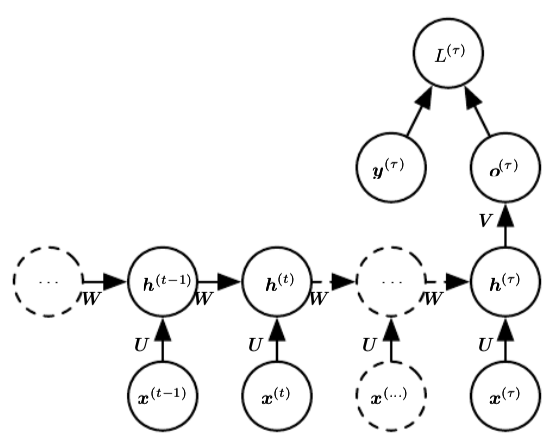
\includegraphics[width=0.45\textwidth]{RNN.png}
		\vspace{-2pt}
		\label{RNN}
		\caption{\textbf{RNNs. $h$=state, $x$=input, $y$=gold label, $\sigma(T)$=predicted label, $t$=time/index}}
	\end{wrapfigure}
	
	\textit{Recurrent Neural Networks} are applied to the word embeddings. \textit{RNN} cells apply the same function (creating a recurrence) to all of the inputs (the embedding vector for each word in the message), while maintaining a hidden internal state that is passed through the recurrence. \cite[p.376]{DL}
	
	This 'state' at any given point is some lossy representation of the past information in the sentence, used to inform the calculations that the model makes at this point. For example, when processing a cyberbullying message, this state could be a notion of context.
	
	The final 'state' of the system is taken and the sigmoid function is applied to get the final output - a number between 0 and 1 representing the probability that the input sentence was a cyberbullying instance or not.
	
	Specificaly, \textit{Long-Short Term Memory} (LSTM) cells are used in this project \cite[p.410]{DL}. Traditional \textit{RNN}s suffer from the vanishing gradient problem. In other words, \textit{RNN}s struggle to learn long-term dependencies in temporal data or text which makes it hard to train them. \textit{LSTM} units introduce a memory cell, which are self-loops, giving them the ability to maintain information for a long time as they process the input data. They can learn what information they should remember and what information they should forget as they train, which means that they typically show much better performance than traditional RNNs.
	
	Bidirectional \textit{LSTM}s are also used in this project. These process sequential data the same in a regular \textit{LSTM}, but both forwards and backwards at the same time. This means that when processing any one word, an \textit{LSTM} cell can use both past and future information to inform decisions at this timestep. This enriches the amount of information that the \textit{LSTM} can draw upon and thus could show an improvement in detecting cyberbullying.
	
	\subsubsection{Convolutional Neural Networks (CNNs)}
	
	\textit{Convolutional neural networks} (CNNs) employ the mathematical operation \textit{convolution}. They allow us to process data with structure, (e.g. 2D images, 3D images, 1D sequences) thus they can be applied to text too \cite[p.330]{DL}.
	
	Convolutions are invariant to translation, and so this allows us to exploit the feature that the same couple of words would indicate cyberbullying, regardless of where in the sentence they occur. For example, '\textit{you d**k}' and '\textit{wow, you d**k}' would both be classed as cyberbullying.
	
	A 1D \textit{Kernel} is defined and moved across the text, followed by a \textit{Pooling} layer which essentially converts the input to an output which is smaller by taking the most prominent features in local areas of the text. \cite[p.339]{DL} 
	
	\textit{CNN}s are utilised in 3 ways in this project:
	\begin{itemize}
		\item \textbf{Traditional \textit{CNN} --- }Numerous \textit{CNN} layers and \textit{Pooling} layers are applied, followed by a traditional dense neural network to eventually classify output into my two classes.
		\item \textbf{\textit{CNN + LSTM} --- }One \textit{CNN} and one \textit{Pooling} layer is applied to reduce feature size and extract some meaningful features of the text. The output from the \textit{Pooling} layer is applied to an \textit{LSTM}. Finally, the \textit{Sigmoid} function is applied to the final state of the \textit{LSTM} cell to classify the sentence.
		\item \textbf{Multi-channel CNN --- }Inspired by Kim \citeyear{Kim}. The idea is that multiple convolutional layers are applied to the input words in parallel with different kernel sizes. The layer outputs are concatenated, and then classified with a \textit{Dense Neural Network}. This is therefore extracting information at different n-gram sizes; groups of words. This idea is illustrated in Figure 3.
	\end{itemize}

	\begin{figure}[h]
		\centering
		\label{multichannel}
		\includegraphics[width=15cm]{"multichannel".png}
		\caption{Multi-channel CNN. NOTE: I apply sigmoid for the 2-class problem, softmax for 3-class.}
	\end{figure}

	\subsubsection{Loss functions}
	\textit{Binary Cross-Entropy} is used as the loss function of the models in this project, and the objective in training a model is to minimise this. However, it also seems logical to maximise the metric being used to evaluate our models (F1 score) directly. Therefore, using ($1-F1$) as the loss function and minimising this, is synonymous with maximising the F1 score of our model. 
	
	This loss function isn't supported by Keras by default, but a custom metric can be designed. F1 must be written using built-in Keras backend functions - this allows the loss function to be differentiable, which is required for backpropagation, thus the network parameters can be shifted accordingly.
	
	In the experimentation phase of this project, both loss functions were used alongside all aforementioned \textit{Deep Learning} architectures and their performance evaluated.
	
	\subsubsection{Regularization}
	In any \textit{Deep Learning} task, the objective is to minimise the generalization error, i.e. to ensure that the model which effectively fits the training data also effectively generalises to unseen test data. There is a danger that overfitting occurs, which is where the training dataset is modelled \textit{too} specifically and so the model demonstrates poor performance on unseen data. 
	
	During experimentation in this project, the following methods of regularization are used:
	\begin{itemize}
		\item \textbf{\textit{Dropout} --- }On each training batch, each cell of the network is removed (activation is set to zero) with a given probability. The loss is therefore backpropagated through a different sub-network for each batch, meaning that over many batches a bagged ensemble of many neural networks is trained. This provides a computationally cheap way of regularising our model \cite[p.273]{DL}. In our RNNs, \textit{Dropout} is applied on the inputs to each cell, however \textbf{\textit{Recurrent Dropout}} can be applied which is where the connections between the recurrent cells are removed at random for each batch, again with a given probability.
		\item \textbf{\textit{Batch Normalization} --- }The layer where \textit{Batch Normalization} is applied is reparametrized which normalizes the activations of each cell across a batch. The primary effect of this is to improve optimization but it can also have a regularizing effect on models in practice \cite[p.1]{Sergey}. 
		\item \textbf{\textit{Early-stopping} --- }When a model is trained long time, it is found that validation error starts to increase after a model starts to overfit to the training data. This means that a model with better generalization is likely to be obtained by saving the parameter setting that achieves the lowest validation set error. When training ceases, these parameters are returned, rather than the latest parameters in training.
	\end{itemize}






\section{Results}
% This section should be between 2 to 3 pages in length.
% This section presents the results of the solutions.  It should include information on experimental settings.  The results should demonstrate the claimed benefits/disadvantages of the proposed solutions.
%\begin{itemize}
%	\item * Measures I decided to use and why. 
%   \item * Differences between F1, MicroF1, WeightedF1, why accuracy and Macro aren't good.
%	\item * Training curves
%	\item * Table with best architecture (with F1 score) for each dataset. Model info.
%	\item * Other interesting settings that I tried with results in same tables
%   \item * Interpret each set of results
%   \item * Comparison between normal loss and F1 loss
%   \itme * 3-class problem! Extension style. Confusion matrix! \newline
%\end{itemize}
\subsection{Evaluation method}
\subsubsection{F1 score}
Once a model has been trained, it is evaluated by observing predictions made on the test set. Throughout this project, F1 score is used as a metric to evaluate the performance of any given \textit{Machine Learning} or \textit{Deep Learning} model. Keeping this metric consistent allows meaningful direct comparison between different models.

The following equations define Precision, Recall and F1 score metrics (TP=number of true positives, FP=number of false positives, FN=number of false negatives). These metrics are more appropriate than accuracy in this project since three of the four datasets contains an imbalanced number of positives and negatives, i.e. most tweets will not be cyberbullying/racism/sexism. Therefore, a high accuracy is achieved if negative is predicted every single time. F1 score ensures that a good balance is achieved; correctly identifying positive examples, but not wrongly identifying cyberbullying too often (predicting 'cyberbullying' every time). As a result, the aim is to maximise F1 score.

\begin{multicols}{2}
	\begin{equation}
	{Precision = \frac{TP}{TP+FP} }
	\end{equation}
	
	\begin{equation}
	{Recall = \frac{TP}{TP+FN} }
	\end{equation}
	
	\begin{equation}
	{F1 = 2 ( \frac{Precision*Recall}{Precision+Recall} )}
	\end{equation}
\end{multicols}

\subsubsection{Training curves}
\begin{wrapfigure}{R}{8cm}
	\centering
	%	\rule{3cm}{7cm}
	% \vspace*{-20pt}
	\includegraphics[width=9cm]{"1K-LSTM32 graph".png}
	\caption{\textbf{Example training graph, LSTM on \textbf{Twitter\_small} dataset}}
	\label{training}
\end{wrapfigure}

In the 3-class problem, F1 score isn't defined this way since there isn't a simple notion of 'positive' and 'negative' instances. For the \textbf{Twitter\_big\_3class} problem, SOTA is calculated as a weighted-macro F1 score \cite{Badjatiya}. This is synonymous with the micro F1 score provided by Sklearn. One method of calculating this is to calculate the F1 score independently for each of the 3 classes, by treating one class at a time as positive and every other instance as negative. The average of the 3 F1 scores is calculated, weighted by the number of instances in that class. In the 3-class problem, the weighted macro F1 score is used.

\textit{Deep Learning} training is much more complex than traditional \textit{Machine Learning}. Firstly, there are many more network parameters to tune. Secondly, these models train over many epochs, shifting their weights with each batch to fit the training data. Accuracy, f1 score and loss can all be observed over time to help infer things about the current model architecture.

As a result, the training accuracy, training loss, validation accuracy  and f1 score on the validation set were calculated at the end of each epoch when training my \textit{Deep Learning} models, and plotted on a graph - these are known as training curves. From these, it is inferred where the maximum performance is achieved (which epoch's parameters were saved with \textit{Early-stopping}) and if a model is overfitting or underfitting - changes to the model can be made accordingly. For example, in Figure \ref{training} it can be seen that the model is overfitting after approximately 60 epochs as the test accuracy starts to go down and the generalization error becomes significant.

%\begin{figure}[H]
%	\centering
%	\label{training}
%	\includegraphics[width=10cm]{"1K-LSTM32 graph".png}
%	\caption{Example training graph, LSTM on \textbf{Twitter\_small} dataset}
%\end{figure}


\subsection{Final Results (2-class Problem)}
In this subsection, the results from \textit{Machine Learning} and \textit{Deep Learning} experimentation on the 2-class datasets are shown. The \textbf{Reddit} and \textbf{Twitter\_small} datasets distinguish between Cyberbullying and not-Cyberbullying. Conversely, the \textbf{Twitter\_big\_2class} dataset's positive class contains a combination of Racist and Sexist comments and the negative class contains tweets that fall under neither sexism nor racism. 

The F1 scores shown are those achieved through the predictions on the test dataset.

\begin{table}[H]
	\centering
	\vspace*{-18pt}
	\caption{Results on \textbf{Reddit} dataset}
	\label{results1}
	\hspace*{-0.8cm}
	\begin{tabular}{p{3.4cm} p{10cm} p{3cm}} \hline\hline
		& \textbf{Model} & \textbf{F1 score}  \\ \hline
		
		\textbf{Machine Learning} & Average GloVe vector + SVM & 0.7147 \\
		& Term Counts + SVM & 0.7288 \\
		& TF-IDF + Multinomial Naive Bayes & 0.7318 \\ 
		& TF + Logistic Regression & 0.7332 \\
		& TF-IDF + Logistic Regression & \textbf{0.7450} \\ \hline
		
		\textbf{Deep Learning} & GloVe + CNN + LSTM + Dropout & 0.7533 \\
		& ELMo + LSTM (300 units) + Dropout & 0.7604* \\
		& GloVe + LSTM (400 units) + Dropout & 0.7620 \\
		& GloVe + LSTM (500 units) + Dropout & \textbf{0.7645} \\ \hline
	\end{tabular}
\end{table}

* due to the computational resources that a large dataset requires to use \textit{ELMo}, inputs were padded to length 100 rather than 500 and only 20K of the 69K dataset examples were used. \newline

This table illustrates that on the \textbf{Reddit} dataset, the performance of \textit{Deep Learning} did exceed that of \textit{Machine Learning} by approximately 2\%. The previous state of the art for \textit{this} dataset was 0.61, and this has been beaten by far. It is interesting to observe that \textit{ELMo} representations are not part of the highest performing model, yet they do come very close at 0.7604 F1 compared to the best \textit{GloVe} model which achieved 0.7645 F1. Perhaps, given greater computational power and then increasing the capacity of the \textit{LSTM} and input pad length would have allowed the models to fully exploit the contextual information that \textit{ELMo} provides.

This data isn't hand-tagged, Instead, instances are labelled based on the number of swear words in the comments. Swear words don't necessarily indicate the presence of cyberbullying, meaning the dataset is of a poor quality. Since these inputs need to be truncated for \textit{Deep Learning} models, they might not have been able to infer this simple labelling technique as many swear words will have been cut out - making this task more difficult and potentially a reason for why the performance is good but not exceptional.

\begin{table}[H]
	\centering
	\vspace*{-12pt}
	\caption{Results on \textbf{Twitter\_small} dataset}
	\label{results2}
	\hspace*{-0.8cm}
	\begin{tabular}{p{3.4cm} p{11cm} p{2cm}} \hline\hline
		& \textbf{Model} & \textbf{F1 score}  \\ \hline
		\textbf{Machine Learning} & TF-IDF + Gradient Boosted Classifier & 0.7253 \\
		& Positives repeated in data + TF + Logistic Regression & 0.7253 \\
		& Positives repeated in data + Term Counts + Logistic Regression & 0.7263 \\
		& Average GloVe vector + Gradient Boosted Classifier & 0.7342 \\
		& Positives repeated in data + TF + Gradient Boosted Classifier & \textbf{0.7978} \\ \hline
		
		\textbf{Deep Learning} & ELMo + LSTM (256 units) & 0.7784 \\
		& Trained word embeddings + LSTM (50 units) + Dropout & 0.7789 \\
		& GloVe + LSTM (100 units) + Dropout & 0.8140 \\ 
		& GloVe + Multi-channel CNN + Batch Normalization & 0.8330 \\ 
		& GloVe + LSTM (150 units) + Dropout & \textbf{0.8372} \\\hline
	\end{tabular}
\end{table}

Again, the performance of \textit{Deep Learning} models has exceeded that of the \textit{Machine Learning} models, this time by approximately 4\%. Interestingly, the highest-performing \textit{Machine Learning} model makes use of repeating positive examples in the dataset. The reasoning is that the model had more motivation to fit ot the positive examples, reducing any overfitting that might occur to the negative class. Furthermore, the Multi-Channel \textit{CNN} method gave some of the best \textit{Deep Learning} results, which shows the effectiveness of combining parallel convolutions. 

Finally, 0.8372 F1 is extremely high and provides evidence to conclude that cyberbullying has effectively been detected. The performance is much better than that on the Reddit dataset. This could be due to the fact that this is a much smaller dataset, which has been collected based on keyword around sexuality, appearance, culture etc. This reduces the feature space as messages are in a similar context - meaning it might be a simpler dataset to model.


\begin{table}[H]
	\centering
	\vspace*{-12pt}
	\caption{Results on \textbf{Twitter\_big\_2class} dataset}
	\label{results3}
	\hspace*{-0.8cm}
	\begin{tabular}{p{3.4cm} p{11cm} p{2cm}} \hline\hline
		& \textbf{Model} & \textbf{F1 score}  \\ \hline
		
		\textbf{Machine Learning} & Term Counts + Logistic Regression & 0.7405  \\
		& Term Counts + Multinomial Naive-Bayes & 0.7421  \\
		& TF-IDF + Bernoulli Naive-Bayes & 0.7424  \\
		& TF + Bernoulli Naive-Bayes & \textbf{0.7551} \\ \hline
		
		\textbf{Deep Learning} & ELMo + Bidirectional LSTM (512 units) + Dropout & 0.7141 \\
		&  One-hot inputs + Multi-channel CNN & 0.7430 \\
		&  Trainable GloVe + LSTM (100 units) + Dropout & 0.7515  \\  
		&  GloVe + LSTM (150 units) + Dropout & 0.7645  \\
		&  GloVe + LSTM (50 units) + Dropout & \textbf{0.7716} \\ \hline
	\end{tabular}
\end{table}

From the 2-class problem results, one can observe that our models are performing at quite a high level, beating the identified state of the art 0.75 F1 \cite{Hack} for a similar problem. However, it is now clear that exact results achieved are dataset dependent, varying approximately 7\% between datasets in this project. The performance is comparable with that of the Reddit dataset, meaning that combining racism and sexism classes doesn't make the presence of hate-speech any more difficult to detect than simply general cyberbullying.

Furthermore, on all three datasets, a simple \textit{LSTM} model with \textit{Dropout} performs reliably well, meaning that good results are obtainable with little experimentation.

\subsection{Further Analysis}
\subsubsection{Binary Cross-Entropy Loss vs F1 loss}
As mentioned in the Solution, Binary Cross-Entropy is used as the loss function for the majority of experimentation in this project - which means the Cross-Entropy is being minimised between the test labels and test predictions. However, since F1 score is the metric being used to evaluate the models' performance, there is motivation to attempt to maximise the F1 score directly. $(1-F1\_score)$ is implemented as a custom loss function and then minimised. 

The best results with each loss function are as follows:

\begin{table}[H]
	\centering
	\vspace*{-10pt}
	\caption{Binary Cross-Entropy vs F1 loss function}
	\label{F1Loss}
	\hspace*{-2.0cm}
	\begin{tabular}{p{3.2cm} p{9cm} p{3.9cm} p{1.7cm}} \hline\hline
		\textbf{Dataset} & \textbf{Model} & \textbf{Loss function} & \textbf{F1 score}  \\ \hline
		
		\textbf{Reddit} & GloVe + LSTM (500 units) + Dropout & Binary Cross-Entropy & 0.7645  \\
		& GloVe + Bidirectional LSTM (400 units) + Dropout & Custom $(1-F1)$ & 0.6707  \\ \hline
		
		\textbf{Twitter\_small} & GloVe + LSTM (150 units) + Dropout & Binary Cross-Entropy & 0.8372 \\
		& GloVe + Multi-Channel CNN + Batch Normalization & Custom $(1-F1)$ & 0.7227 \\ \hline
		
		\textbf{Twitter\_big\_2class} & GloVe + LSTM (50 units) + Dropout & Binary Cross-Entropy & 0.7716 \\
		& GloVe + Bidirectional LSTM (50 units) + Dropout & Custom $(1-F1)$ & 0.7535 \\ \hline
	\end{tabular}
\end{table}

In no case does directly maximising F1 increase the model's performance on the test data. 

However, Figure \ref{train:train2} shows 2 training graphs on the \textbf{Twitter\_big\_2class} dataset. The left shows an \textit{LSTM} applied with Cross-Entropy loss, the second shows a Bidirectional \textit{LSTM} applied with custom $(1-F1)$ loss; the best results achieved with the respective loss functions on this dataset. There is little difference between the two graphs, except that the generalization error is larger with Cross-Entropy loss, which is inferred from the larger gap between the train and test accuracy curves. Perhaps, directly maximising F1 score is informing the model to prioritise generalization across the 2 classes rather than overfitting to one class.

\begin{figure}[H]
	\centering
	% \hspace*{-0.10\textwidth}
	\includegraphics[width=.45\textwidth]{"lstm_train".png} \hfill
	\includegraphics[width=.45\textwidth]{"f1_train".png}\hfill
	%\hspace*{-0.10\textwidth}
	
	\caption{Training curves on \textbf{Twitter\_big\_2class}. \textbf{Left:} Cross-Entropy loss, \textbf{Right:} F1 loss.}
	\label{train:train2}
\end{figure}

Although there was no increase in performance here, it was an interesting experiment.

\subsubsection{3-class problem}

With success in the 2-class problem, experimentation continued around the 3-class problem on the \textbf{Twitter\_big\_3class} dataset, with classes Racism, Sexism and Neither Racism nor Sexism. The aim was to beat the state of the art for this problem, 0.93 weighted-macro F1 \cite{Badjatiya}. Categorical Cross-Entropy is used as the loss function, since there are 3 classes.

\begin{table}[H]
	\centering
	\vspace*{-12pt}
	\caption{Results on \textbf{Twitter\_big\_3class} dataset}
	\label{results4}
	\hspace*{-1.5cm}
	\begin{tabular}{p{3.4cm} p{10.5cm} p{3.8cm}} \hline\hline
		& \textbf{Model} & \textbf{Weighted Macro F1}  \\ \hline
		
     \textbf{Machine Learning} & Trigrams + SVM & 0.8342 \\
	& Trigrams + Gradient-Boosted Classifier & 0.8377 \\
	& TF + Logistic Regression & 0.8399 \\
	& TF + Bernoulli Naive Bayes & 0.8408 \\
	& Term Counts + Logistic Regression & \textbf{0.8465} \\ \hline
	
	\textbf{Deep Learning} & Trainable GloVe + LSTM (100 units) + Dropout & 0.8370  \\  
	& GloVe + Bidirectional LSTM (100 units) + Dropout & 0.8384  \\
	& ELMo + LSTM (256 units) + Dropout & 0.8394  \\
	& GloVe + LSTM (50 units) + Dropout + Batch Normalization & 0.8411 \\ 
	& ELMo + LSTM (512 units) + Dropout & \textbf{0.8419} \\ \hline
	\end{tabular}
\end{table}

Interestingly, in the 3-class problem there is no differentiation between the performance of our \textit{Machine Learning} and \textit{Deep Learning} models; there are a large number of completely differently models all achieving weighted macro f1 approximately 0.84.

Confusion matrices allow visualisation of a model's predictions against the test labels. Figure \ref{CM:CM2} shows an example of a confusion matrix for a well-performing model in the 2-class and 3-class tasks for the \textbf{Twitter\_big} dataset. A reminder that \textbf{Twitter\_big\_2class} is the same dataset as \textbf{Twitter\_big\_3class} but with the sexism and racism classes combined.

\begin{figure}[H]
	\centering
	% \hspace*{-0.10\textwidth}
	\includegraphics[width=.25\textwidth]{"2class_CM".png} 
	\hspace*{0.05\textwidth}
	\includegraphics[width=.35\textwidth]{"3class_CM".png}
	\vspace*{-0.5cm}
	%\hspace*{-0.10\textwidth}

	\caption{Confusion matrices. \newline\textbf{Left:} 2-class problem, \textbf{Right:} 3-class problem (0=None, 1=Racism, 2=Sexism)}
	\label{CM:CM2}
\end{figure}

The 2-class matrix shows that misclassification occurs both ways, our model often predicting positive instead of negative and vice versa. However, the 3-class matrix shows that although the model often wrongly predicts 0/None instead of racism or sexism and vice versa, the model almost never misclassifies between racism and sexism classes, only 0.1\% of examples being classified as sexism instead of racism, and 0.2\% as racism instead of sexism.

From this, it is concluded that \textit{Deep Learning} models are much more effective at distinguishing between the different \textit{types} of hateful speech, as opposed to detecting in a binary task whether hateful speech is present or not.


\section{Evaluation}
% This section should between 1 to 2 pages in length.
%\begin{itemize}
%	\item * Strengths and Weakness of solution
%  		 \item * Compromises with Dixon dataset, resources 
%   	 \item * This is research, beating SOTA not TOO important
%	\item * Lessons learnt
%   	  \item * Is DL worth it? \newline
%\end{itemize}

\subsection{Strengths and Limitations}
Firstly, due to a rapid increase in interest \textit{Deep Learning} is becoming an extremely popular field of research. The most important thing in this project, aside from trying to beat the state of the art performance for this task, was providing research into this topic with cutting edge or completely new ideas. For example, \textit{ELMo} representations formed a core part of the experimentation in this project; the results illustrating their potential strengths, achieving reliably good results on all datasets and the \textit{best} results on the \textbf{Twitter\_big\_3class} dataset. Additionally, \textit{directly} maximising the F1 score as part of the loss function was an intriguing idea - not necessarily improving results but demonstrating good generalisation and providing a potential idea for future research.

State of the Art for the 2-class problem is 0.75 \cite{Hack}, and 0.8372 was achieved on the \textbf{Twitter\_small} dataset. However it must be considered that results are somewhat dependent on the dataset, so a concrete comparison can not be made as the \#HackHarrassment dataset is not publicly available. 

Unfortunately, a limitation to the project was that the 3-class State of the Art, 0.930 \cite{Badjatiya} was not beaten (0.8419 was achieved), however, observing that models can distinguish between \textit{types} of hate-speech more than they can detect the \textit{presence} of hate-speech is a valuable insight.

Another limitation to the project is that compromises were made on the Reddit dataset. It is a vast dataset, with 69K examples up to 2500 words long. As a result, examples were truncated to 500 words and when using the feature-rich \textit{ELMo} representations, these were truncated to just 100 words and only 20K examples were used. Given better computational resources with more memory, additional information could be exploited and perhaps performance would be improved. 

A huge variety of models were used in this research. 10 different traditional \textit{Machine Learning} models were implemented, each tuned on 7 different feature representations. Many \textit{Deep Learning} architectures were implemented too; 4 different input representations, various \textit{Recurrent Neural Networks} and \textit{Convolutional Neural Network} setups, each tuned and regularized. All of this research was conducted over 4 different datasets to provide in depth insight into the importance of data in a problem of this nature. 


\subsection{Is Deep Learning worth it?}
% \lipsum[1-4]
\begin{wrapfigure}{R}{6cm}
	\centering
	%	\rule{3cm}{7cm}
	\vspace{-30pt}
	\includegraphics[width=.45\textwidth]{"MLvsDL".png} 
	\caption{\textbf{The importance of dataset size for ML and DL performance.}}
	\label{MLvsDL}
\end{wrapfigure}

Although not the case in the 3-class problem, where \textit{Machine Learning} performed marginally better, it can be concluded that \textit{Deep Learning} models exceed the performance of traditional \textit{Machine Learning} for the 2-class problem when detecting Cyberbullying, since for all three 2-class datasets, there is a 0.0195, 0.0333 and 0.0394 increase in the best f1 score achieved respectively. 

However, \textit{Deep Learning} architectures are far more varied, contain more network parameters and the time and computational resources required for experimentation are far greater than that of simple traditional \textit{Machine Learning} models. This extra difficulty must be considered for what is a relatively marginal (approx. 3\% on average) performance increase.

Additionally, the amount of data affects the difference in \textit{Machine Learning} and \textit{Deep Learning} performance. Figure \ref{MLvsDL} illustrates the difference here \cite{BuildDeeper}. The improvement of \textit{Deep Learning} performance over \textit{Machine Learning} (approximately 3\% on the 2-class problem), suggests that \textit{Machine Learning}'s 'Plateau in Performance' is yet to be reached. As a result, a larger dataset for this task would be likely to increase the value of \textit{Deep Learning}'s experimentation.


\subsection{The Importance of Data}

A good dataset is vital in \textit{Machine Learning} and \textit{Deep Learning} tasks. The maximum F1 achieved in this project varied by approximately 7\% between datasets, despite extensive architecture experimentation and in-depth model-tuning. This shows how reliant our models are on good underlying data. 

For example, the Reddit dataset automatically tags comments based on swear word count which is unreliable, meaning that the semantics of an instance might not actually correlate with the label. This limited the performance in models for this dataset. Contrary to this, the Twitter\_small dataset consists of only 1,066 instances, collected based on a limited keyword search. This is likely to limit the feature space, perhaps making this an easier task - leading to the impressive F1 of 0.8372 that was achieved.






\section{Conclusion}
% This section summarises the main points of this paper.  Do not replicate the abstract as the conclusion.  A conclusion might elaborate on the importance of the work or suggest applications and extensions.  This section should be no more than 1 page in length.
%\begin{itemize}
%	\item * What I have achieved overall
%   \item * DL worth it?
%	\item * Better at differentiating between types of hateful language than detecting presence or not.
%	\item * Future work (more CPU power, bigger dataset) \newline
%\end{itemize}
In this project, it has been concluded that \textit{Deep Learning} is able to perform better than \textit{Machine Learning} in the 2-class problem, an improvement of approximately 3\% when experimenting with Deep Methods. However, the extra running time and computational resources that are required to create and tune an effective \textit{Deep Learning} model require consideration - as illustrated by the compromises made on the Reddit dataset that limited \textit{Deep Learning} performance. 

As inferred from the findings in the 3-class problem, \textit{Deep Learning} models are much better at distinguishing between types of hate-speech (namely, sexism and racism) than they are at detecting the actual presence of hate-speech. Additionally, the potential for using the cutting-edge \textit{ELMo} word representations has been illustrated, achieving some of the best results in this project.

Finally, good data is vital to a high-performing \textit{Deep Learning} model, as observed from the difference in results across datasets. No perfect dataset exists online that is large enough, and nobody would want to collect this data themselves due to the offensive nature of the task. This may limit the potential for future research in this subject area.

\subsection{Future work}
Further to the compromises made on the Reddit dataset, it would be ideal to obtain greater computational resources and experiment with \textit{Deep Learning} methods on the entire dataset, with no truncation of inputs. An insight could be gained into whether more information would lead to greater results - I believe that this would be the case.

Secondly, from Figure \ref{MLvsDL}, it can be observed that a larger dataset would likely lead to improved results. A logical extension to this research would be to collect a much larger dataset, but as mentioned, the offensive messages provide a strong deterrent. A workaround could be to collect as many publicly available datasets as possible and concatenate them together. It would be extremely interesting to see if this improves the results when compared to each dataset seaparately as in this project.




%\begin{table}[htb]
%\centering
%\caption{SUMMARY OF PAGE LENGTHS FOR SECTIONS}
%\vspace*{6pt}
%\label{summary}
%\begin{tabular}{|ll|c|} \hline
% & \multicolumn{1}{c|}{\bf Section} & {\bf Number of Pages} \\ \hline
%I. & Introduction & 2--3 \\ \hline
%II. & Related Work & 2--3 \\ \hline
%III. & Solution & 4--7 \\ \hline
%IV. & Results & 2--3 \\ \hline
%V. & Evaluation & 1-2 \\ \hline
%VI. & Conclusions & 1 \\ \hline
%\end{tabular}
%\end{table}



%\subsection{References}

% The list of cited references should appear at the end of the report, ordered alphabetically by the surnames of the first authors.  References cited in the main text should use Harvard (author, date) format.  When citing a section in a book, please give the relevant page numbers, as in \cite[p293]{budgen}.  When citing, where there are either one or two authors, use the names, but if there are more than two, give the first one and use ``et al.'' as in  , except where this would be ambiguous, in which case use all author names.

% You need to give all authors' names in each reference.  Do not use ``et al.'' unless there are more than five authors.  Papers that have not been published should be cited as ``unpublished'' \cite{euther}.  Papers that have been submitted or accepted for publication should be cited as ``submitted for publication'' as in \cite{futher} .  You can also cite using just the year when the author's name appears in the text, as in ``but according to Futher \citeyear{futher}, we \dots''.  Where an authors has more than one publication in a year, add `a', `b' etc. after the year.


\bibliography{projectpaper} 



\end{document}